% based on IEEE template, adapted by Tim Bruedigam and students
\documentclass[conference]{IEEEtran}
\IEEEoverridecommandlockouts
%%%%%%%%%%%%%%%%%%%%%%%%%%%%%%%%%%%%%%%%%%%%%%%%%%%%%%%%%%%%%%
% CUSTOMIZING Tex-File for students to be adjusted as needed %
%%%%%%%%%%%%%%%%%%%%%%%%%%%%%%%%%%%%%%%%%%%%%%%%%%%%%%%%%%%%%%
%%%%%%%%%%%%%%%%%%%%%
% CUSTOM PACKAGES	%
%%%%%%%%%%%%%%%%%%%%%
\usepackage{tikz}
\usepackage{pgfplots}

% \usepackage{IEEEtrantools}

%%%%%%%%%%%%%%%%%%%%%
% CUSTOM COMMANDS	%
%%%%%%%%%%%%%%%%%%%%%
% e.g. Math conventions as vectors, Matrices, sets
\renewcommand{\vec}[1]{\mathbf{\MakeLowercase{#1}}}
\newcommand{\Mat}[1]{\mathbf{\MakeUppercase{#1}}}
\newcommand{\set}[1]{\boldsymbol{#1}}

% e.g. use differenc layers in tikz
\pgfdeclarelayer{background}
\pgfdeclarelayer{nodelayer}
\pgfdeclarelayer{edgelayer}
\pgfdeclarelayer{foreground}
\pgfsetlayers{background,edgelayer,nodelayer,main,foreground}
%%%%%%%%%%%%%%%%%%%%%
% HYPHENATIONS 		%
%%%%%%%%%%%%%%%%%%%%%
\hyphenation{Lya-pu-nov}


% %%%%%%%%%%%%%%%%%%%%%%%%%%%%%%%%%%%%%%%%%%%%%%%%%%%%%%%%%%%%%%
% NOTE: Using this is optional
% 	Nonetheless, feel free to include this file and adjust the 
% 	examples below as needed
%   
% Questions, feedback and improvements:
%	-> https://git.lsr.ei.tum.de/students/student-templates/issues
% ATTENTION:
% 	- Keep in mind that thif file uses the \vec and \mat commands
% 	 	which are defined in customize.tex!
%	- add glsaddall if you want all of the elements in gloss.aux
%		being printed into your list of acronyms.
% Further reading:
%	https://ctan.org/pkg/glossaries?lang=en
%%%%%%%%%%%%%%%%%%%%%%%%%%%%%%%%%%%%%%%%%%%%%%%%%%%%%%%%%%%%%%

% include packages
\usepackage{setspace}
\usepackage{filecontents}
% for sharelatex, the indexing using xindy:
% 	http://xindy.sourceforge.net/doc/faq-1.html#ss1.2
% is not available, thus the adjustments below ar necessary
%% Adjust Flag for Sharelatex
\newif\ifShareLatex 
%\ShareLatextrue            	% if you work in sharelatex: https://sharelatex.tum.de
\ShareLatexfalse          		% if you work locally

\ifShareLatex
    \usepackage[acronym, style=alttree, shortcuts, toc=true, nomain, nonumberlist]{glossaries}
    \renewcommand{\makeglossaries}{\makenoidxglossaries}
    \renewcommand{\printglossary}{\printnoidxglossary}
\else
    \usepackage[acronym,style=alttree, toc=true, shortcuts, xindy, nomain, nonumberlist]{glossaries}
    \RequirePackage[xindy]{imakeidx}
\fi

%%%%%%%%%%%%%%%%%%%%%%%%%%%%%%%%%%
% DEFINE HEADINGS AND CATEGORIES %
%%%%%%%%%%%%%%%%%%%%%%%%%%%%%%%%%%
% preferable use a command, to adjust the Capitalization 
% for the header section of fancyhdr automatically
\newcommand{\Symbols}{List of Symbols}
\newcommand{\Notation}{Notation}
\newglossary{symbols}{sym}{sbl}{\Symbols}
\newglossary{notation}{not}{nt}{\Notation}
% set width of first row
\glssetwidest{THISWIDE}     % adjust length as needed

%%%%%%%%%%%%%%%%%%%%%%%%%%%%%
% DEFINE ACRONYMS/GLOSSARY	%
%%%%%%%%%%%%%%%%%%%%%%%%%%%%%
\makeglossaries % don't remove this
\begin{filecontents}{gloss.aux}
	%===========%
	% ACRONYMS	%
	%===========%
	\newacronym{MPC}{MPC}{model-predictive control}
	\newacronym{BIBO}{BIBO}{bounded-input bounded-output}
	\newacronym{HRC}{HRC}{Human-Robot Collaboration}
	%============%
	% SYMBOLS	%
	%===========%
	\newglossaryentry{control}{type=symbols,
		sort={control},
		name={\ensuremath{\vec{u}}},
		description={control input vector}
	}
    \newglossaryentry{uk}{type=symbols,
		sort={control},
		name={\ensuremath{\vec{u}_k}},
		description={control input vector with time step}
	}
    \newglossaryentry{xk}{type=symbols,
		sort={state},
		name={\ensuremath{\vec{x}_k}},
		description={state vector with time step}
	}
	%============%
	% NOTATION	%
	%===========%
	\newglossaryentry{vector}{type=notation,
		sort={vector},
		name={\ensuremath{\vec{x}_n}},
		description={$n$-dimensional vector named $x$}
	}	
	\newglossaryentry{matrix}{type=notation,
		sort={vector-matrix},
		name={\ensuremath{\Mat{x}_{m\times n}}},
		plural={matrices},
		user1={Mat},
		description={\ensuremath{m\times n} dimensional Matrix  named \ensuremath{X}}
	}	
\end{filecontents}
\loadglsentries{gloss.aux}

%%%% Add GLOSSARIES at end of thesis
\newcommand{\AddMyGloss}{
	\renewcommand{\glsglossarymark}[1]{}
   	\printglossary[type=acronym]
	\markboth{\MakeUppercase{acronyms}}{\MakeUppercase{acronyms}}
  	\ifdefined\Symbols
		\printglossary[type=symbols, nogroupskip]
		\markboth{\MakeUppercase{\Symbols}}{\MakeUppercase{\Symbols}}
	\fi
	\ifdefined\Notation
		\printglossary[type=notation, nogroupskip]
		\markboth{\MakeUppercase{\Notation}}{\MakeUppercase{\Notation}}
	\fi
}

		% add your glossary in this file 

%\usepackage{cite}
\usepackage{float}
\usepackage{caption}
\usepackage{subcaption}
\usepackage{amsmath,amssymb,amsfonts}
\usepackage{algorithmic}
\usepackage{graphicx}
\usepackage{textcomp}
\usepackage{diagbox}
%\usepackage[utf8]{inputenc}
\newcommand{\chapter}{\section}
%\def\BibTeX{{\rm B\kern-.05em{\sc i\kern-.025em b}\kern-.08em
%    T\kern-.1667em\lower.7ex\hbox{E}\kern-.125emX}}
\begin{document}



%%%%%%%%%%%%%%%%%%%%%%%%%%%%% Title / Student %%%%%%%%%%%%%%%%%%%%%%%%%%%%%%%%
\title{Numerical Discretization in High Accuracy MPC Applications
}

\author{\IEEEauthorblockN{Tianyuan Kong}
\IEEEauthorblockA{\textit{Department of Electrical and Computer Engineering, Chair of Automatic Control Engineering (LSR)} \\
\textit{Technical University of Munich}\\
Munich, Germany\\
ge23loy@tum.de}
}

\maketitle


%%%%%%%%%%%%%%%%%%%%%%%%%%%%% Document %%%%%%%%%%%%%%%%%%%%%%%%%%%%%%%%
\begin{abstract}
This work provides a comparative review of numerical methods generally used to discretize continuous-time linear system models appearing in Model Predictive Control (MPC) problems, i.e., Runge-Kutta (RK) methods and Gauss collocation. An overview of the characteristics of different RK methods, i.e. RK1, RK2, RK4, are given and the performance of each method is evaluated in a simulation example. Furthermore, we provide a discretization method based on Gauss collocation that allows to consider piecewise polynomial input functions within MPC, akin to higher-order hold elements.
\end{abstract}

\begin{IEEEkeywords}
discretization methods, model predictive control, Runge-Kutta methods, Gauss collocation, real-time optimization
\end{IEEEkeywords}


%_________Einleitung__________________________________
\chapter{Introduction}
\label{sec:introduction}

MPC is a control technique that uses models of the plant in order to predict the future behaviour of the system over a prediction horizon. Usually, these models are expressed mathematically as ordinary differential equations (ODE) \cite{sanchez2017mpc}. Applying MPC schemes to continuous time systems requires numerical
discretization of the continuous time optimal control problem. Commonly used discretization approaches for MPC are based on RK methods. For the implementation in a sampled control loop, typically zero-order hold (ZOH), i.e., piecewise constant inputs between the sampling intervals are used. In applications where the continuous time model is exactly known and high accuracy control is required, a finer discretization grid or a higher order RK method can be chosen to decrease the
approximation error of the discretization method, e.g., Gauss collocation \cite{kotyczka2021high} with appropriate higher-order hold elements.

\section{Problem Statement}

 The goal of this work is to derive a trade-off between prediction accuracy and computational complexity within an MPC scheme for continuous time linear systems. This is investigated by varying the granularity of numerical discretization and the order of RK methods, including the order of the hold element in the sampled control loop. In addition, the effects of the discretization approaches on the computation of reachable and invariant sets are also examined. Results from this work will enable similar investigations for the sampled control of continuous time nonlinear systems by MPC schemes.  In MPC, higher accuracy of the discretization leads to increased computational load as more decision variables are introduced to the optimal control problem, which can result in infeasible computation time.



%____________________________________________________
%\chapter{Problem Setup}
\section{Problem Setup}
In the following we consider a continuous-time dynamical systems described by the following equation
\begin{equation}
	\dot{x} = f(x(t),u(t)),
\end{equation}
where $x(t)\in\mathbb{R}^m $ is the state and $u(t)\in\mathbb{R}^n$ is the control input.
The MPC problem is defined as follows: determine the state $x_k \in \mathbb{R}^m$ and $u_k \in \mathbb{R}^n$ that solves the optimization problem
\begin{equation}
	\begin{split}
	    \min \limits_{(x,u)} \sum_{k=i}^{i+N-1} l_k(x_k,u_k) &+ l_N(x_{k+N})\\
	    s.t. \qquad \qquad  x_i - \bar{x_i} &= 0,\\
	                x_{k+1}-f_k(x_k,u_k) &= 0,\\
	                h_k(x_k,u_k)  &\leq 0,\\
	                \forall k &\in [i, \cdots, i + N-1]   
	\end{split}
\end{equation}
where $N$ is the control horizon, $l_k$ is the stage cost, $l_N$ is the terminal cost (a popular choice is the use of quadratic costs \cite{maciejowski2002predictive}). The parameter $\bar{x_i}$ is the fixed initial value, the function $f_k$ is the discrete-time version of (1), and the function $h_k$ describes state and control constraints. In order to solve (2) we need to find a method to discretize (1), thus allowing to solve a non-linear program (NLP) on the free variables (x,u).

Particularly in this work, we assume a continuous time LTI system with the system matrices $A_{\rm {con}}$ and $B_{\rm {con}}$, the ODE of this system can be represented by the following equation
\begin{equation}
	\dot{x} = A_{\rm {con}}x + B_{\rm {con}}u,
	\label{eq:ode}
\end{equation}
The discrete-time system can be expressed as
\begin{equation}
	x_{k+1} = A_{\rm{d}}x_k + B_{\rm{d}}u_k,
\end{equation}


\chapter{Technical Approach}
In the following, we will discuss methods on how to retrieve a discretized system of the form (4) from a given contunuous-time system equation as in (3). During the analysis of different discretization methods, we firstly introduce the zero-order hold (ZOH), i.e., piecewise constant inputs $u$ between the sampling intervals $\Delta t$, and first-order hold (FOH), i.e., piecewise linear inputs $u$ between the sampling intervals $\Delta t$. The ZOH is illustrated in Fig. \ref{fig:ZOH} and FOH is illustrated in Fig. \ref{fig:FOH}
\begin{figure}[h]
	\centering
	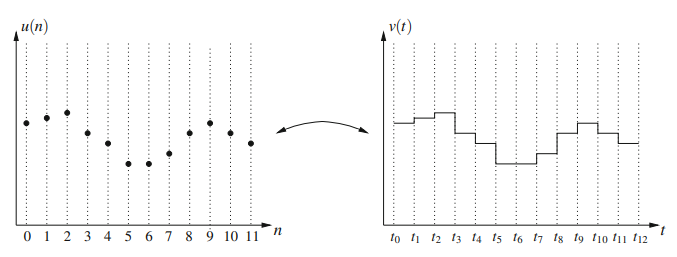
\includegraphics[width=\linewidth]{pics/ZOH.png}
	\caption{Illustration of zero-order hold \cite{grune2017nonlinear}}
	\label{fig:ZOH}
\end{figure}
\begin{figure}[h]
	\centering
	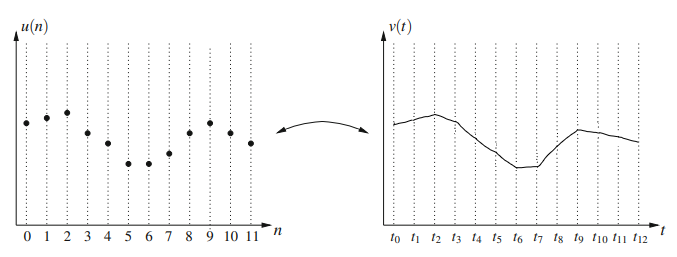
\includegraphics[width=\linewidth]{pics/FOH.png}
	\caption{Illustration of first-order hold}
	\label{fig:FOH}
\end{figure}


\subsection{Runge-Kutta method}
Given a continuous time LTI system in Eq. (\ref{eq:ode}), the corresponding RK discretization models can be represented by the following equation:
\begin{equation}
	x_{k+1} = A_{\rm{rk}}x_k + B_{\rm{rk}}u_k,
	\label{eq5}
\end{equation}

The family of explicit RK methods is given by
\begin{equation}
	x_{k+1} = x_k +  \sum_{i=1}^s b_i \kappa_i,
\end{equation}
where
\begin{equation}
	\begin{split}
		%\frac{dx}{dt} &=  f(t, x), \quad x\left(t_{0}\right)=x_{0},\\
		\kappa_1 &= \Delta t f(t_k,x_k,u_k),\\
		\kappa_2 &= \Delta t f(t_k+c_2\Delta t, x_k+\Delta t(a_{21}\kappa_1),u_k),\\
		\kappa_3 &= \Delta t f(t_k+c_3\Delta t, x_k+\Delta t(a_{31}\kappa_1+a_{32}\kappa_2),u_k)\\
		\vdots\\
		\kappa_s &= \Delta t f(t_k+c_s\Delta t,\\&  \quad x_k+\Delta t(a_{s1}\kappa_1+a_{s2}\kappa_2+\cdots+a_{s,s-1}\kappa_{s-1}),u_k).
	\end{split}
\end{equation}
\\
To specify a particular method, one needs to provide the integer $s$ (the number of stages), and the coefficients $a_{ij}$ (for $1 \leq j <i \leq s$) and $c_i$ (for $i=2,3,\cdots,s$). The matrix consisting of the elements $a_{ij}$, which is called Runge-Kutta matrix, while the $b_i$ and $c_i$ are known as the weights and nodes. More compactly, these parameters are written as so-called Butcher tableaus\cite{grune2017nonlinear} of the form
\begin{table}[H]
  \begin{center}
  	\begin{tabular}{c|l}
  	$c_1$ &  \\
  	$c_2$ & $a_{21}$ \\
  	$c_3$ & $a_{31}$ $a_{32}$\\
  	$\vdots$ & $\vdots$ $\quad$ $\quad$ $\ddots$\\
  	$c_s$ & $a_{s1}$ $a_{s2}$ $\cdots$ $a_{s,s-1}$\\
  	\hline
  	$\quad$ & $b_1\ \ $ $b_2\ $ $\cdots$ $b_{s-1}\ \ $ $b_s$
  	\end{tabular}	
  \end{center}
\end{table}
Table 1 shows Butcher tableaus corresponding to the Euler scheme known as RK1 (left), the Heun scheme known as RK2 (middle) and the so-called classical Runge–Kutta scheme with s = 4 stages proposed by Carl Runge and Martin Kutta in 1895 (right).
\begin{table}[!htb]
	\begin{minipage}{.33\linewidth}
		\caption{}
		\centering
		\begin{tabular}{c|l}
			$0$ &  \\
			\hline
			& 1
		\end{tabular}
	\end{minipage}%
	\begin{minipage}{.33\linewidth}
		\centering
		\caption{}
		\begin{tabular}{c|l}
			$0$ &  \\
			1 & 1  \\
			\hline
			& $\frac{1}{2}$ $\frac{1}{2}$
		\end{tabular}
	\end{minipage} %
    \begin{minipage}{.33\linewidth}
    	\caption{}
    	\centering
    	\begin{tabular}{c|l}
    		$0$ &  \\
    		$\frac{1}{2}$ & $\frac{1}{2}$ \\
    		$\frac{1}{2}$ & $0$ $\frac{1}{2}$\\
    		$1$ & $0$ $0$ $1$            \\
    		\hline
    		& $\frac{1}{6}$ $\frac{2}{6}$ $\frac{2}{6}$ $\frac{1}{6}$
    	\end{tabular}
    \end{minipage}
\end{table}

We solve the MPC problem using numerical optimization methods, therefore the continuous-time dynamical system equations need to be discretized. If control input $u$ is known continuously, then we can directly evaluate $u(t)$ at the given sampling interval of RK method. For example, when using the fourth order Runge-Kutta method with ZOH, using $x_n = x(t_0+n\Delta t)$ and $u_n = u(t_0+n\Delta t)$, then we obtain
\begin{equation}
	\begin{split}
		x_{k+1} &= x_k + \frac{1}{6}(\kappa_1 + 2\kappa_2 +2\kappa_3 + \kappa_4),\\
		\kappa_1 &= \Delta t(A_{\rm{con}}x_k+B_{\rm{con}}u_k),\\
		\kappa_2 &= \Delta t(A_{\rm{con}}(x_k+\kappa_1/2)+B_{\rm{con}}u_k),\\
		\kappa_3 &= \Delta t(A_{\rm{con}}(x_k+\kappa_2/2)+B_{\rm{con}}u_k),\\
		\kappa_4 &= \Delta t(A_{\rm{con}}(x_k+\kappa_3)+B_{\rm{con}}u_k).\\
	\end{split}
\end{equation}
Substituting these equations into each other gives
\begin{equation}
	\begin{split}
	    x_{k+1} &= \underbrace{\left(I + \Delta t A_{\rm{con}} + \frac{{\Delta t}^2}{2!}A_{\rm{con}}^2 + \frac{{\Delta t}^3}{3!}A_{\rm{con}}^3 + \frac{{\Delta t}^4}{4!}A_{\rm{con}}^4\right)}_{\rm{A_{rk4}}}x_k\\
	    &+ \underbrace{\left(\Delta t I  + \frac{{\Delta t}^2}{2!}A_{\rm{con}} + \frac{{\Delta t}^3}{3!}A_{\rm{con}}^2 + \frac{{\Delta t}^4}{4!}A_{\rm{con}}^3\right)B_{\rm{con}}}_{\rm{B_{rk4}}}u_k.
	\end{split}
\end{equation}
Therefore, the system matrices $A_{\rm{rk}}$ and $B_{\rm{rk}}$ in (5) are:
\begin{equation}
	\begin{split}
		A_{\rm{rk4}} &= I + \Delta t A_{\rm{con}} + \frac{{\Delta t}^2}{2!}A_{\rm{con}}^2 + \frac{{\Delta t}^3}{3!}A_{\rm{con}}^3 + \frac{{\Delta t}^4}{4!}A_{\rm{con}}^4,\\
		B_{\rm{rk4}} &= \left(\Delta t I  + \frac{{\Delta t}^2}{2!}A_{\rm{con}} + \frac{{\Delta t}^3}{3!}A_{\rm{con}}^2 + \frac{{\Delta t}^4}{4!}A_{\rm{con}}^3\right)B_{\rm{con}}.
	\end{split}
\end{equation}
Similar to RK4 approximation, we can obtain the system matrices of RK1 and RK2 methods:
\begin{equation}
	\begin{split}
		A_{\rm{rk1}} &= I + \Delta t A_{\rm{con}},\\
		B_{\rm{rk1}} &= \Delta tB_{\rm{con}},\\
		A_{\rm{rk2}} &= I + \Delta t A_{\rm{con}} + \frac{{\Delta t}^2}{2!}A_{\rm{con}}^2,\\
		B_{\rm{rk2}} &= \left(\Delta t I  + \frac{{\Delta t}^2}{2!}A_{\rm{con}}\right)B_{\rm{con}}.
	\end{split}
\end{equation}

\subsection{Gauss collocation method}
Using $s$-stage Gauss collocation, we can get the numerical approximation of the discrete-time model. 
The Gauss collocation numerical solution with state stage values $x_{k}^{o, i}$, $i = 1,...,s$:
\begin{equation}
	\begin{split}
		{x}_{k+1} &={x}_{k}+ \Delta t \sum_{i=1}^{s} b_{i}^{s} \mathbf{f}\left(\mathbf{x}_{k}^{o, i}\right)+\Delta t \mathbf{g} \sum_{i=1}^{s} b_{i}^{s} u_{k}^{i} ,\\ {x}_{k}^{o, i} &={x}_{k}+\Delta t \sum_{j=1}^{s} a_{i j}^{s} \mathbf{f}\left(\mathbf{x}_{k}^{o, j}\right)+\Delta t \mathbf{g} \sum_{j=1}^{s} a_{i j}^{s} u_{k}^{j} ,
	\end{split}
\end{equation}
where the RK coefficients $a_{i j}^{s} =\int_{0}^{c_{j}} \ell_{i}^{s-1}(\tau) d \tau$ and $b_{i}^{s} =\int_{0}^{1} \ell_{i}^{s-1}(\tau) d \tau$.
In Gauss collocation method, the control input $u_k$ can be shaped with Lagrange polynomials. The control input for $t \in\left[t_{k}, t_{k+1}\right)$ generated via an $s-1$ order hold element using Lagrange interpolation polynomials \cite{kotyczka2021high}:
\begin{equation}
	u\left(t_{k}+\tau \Delta t\right)=\sum_{i=1}^{s} u_{k}^{i} \ell_{i}^{s-1}(\tau),
\end{equation}
where $$
\ell_{i}^{s-1}(\tau)=\prod_{\substack{l=1 \\ l \neq i}} \frac{\tau-c_{l}}{c_{i}-c_{l}}.
$$
The control stage values in the collocation points (weights of Lagrange polynomials):
$$
u\left(t_{k}^{i}\right)=u_{k}^{i}, \quad t_{k}^{i}=t_{k}+c_{i} \Delta t, \quad i=1, \ldots, s
$$
The collocation points on the unit interval are shown in Fig.~\ref{fig:gausscoll}, the collocation points $c_{1}^{0}=\frac{1}{2}$ and $c_{1 / 2}^{1}=\frac{1}{2} \mp \frac{\sqrt{3}}{6}$
\begin{figure}[h]
	\centering
	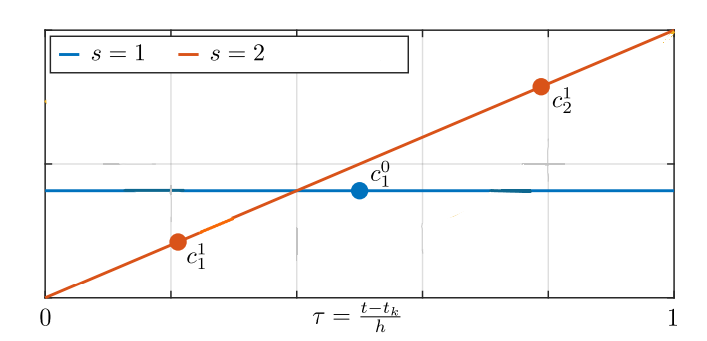
\includegraphics[width=\linewidth]{pics/gausscoll.png}
	\caption{Control signal shapes on the unit interval based on Gauss collocation points}
	\label{fig:gausscoll}
\end{figure}
\\\\
Given the same continuous time LTI system in (\ref{eq:ode}), the corresponding Gauss collocation discretization models can be represented by an equation of the form (4).
\subsubsection{Zero-order hold control input}
When $s = 1$, i.e. the zero-order hold case, the control input for $t \in \left[t_k, t_{k+1}\right]$ results in
$$u(t) = u_k$$
\\
The exact discretization model can be represented as:
\begin{equation}
	x_{k+1} = A_{\rm{ex,1}}x_k+B_{\rm{ex,1}}u_k,
\end{equation}
where $A_{\rm{ex,1}} = e^{A_{\rm{con}}  \Delta t}$ and $B_{\rm{ex,1}} = \int_{0}^{\Delta t} e^{A_{\rm{con}}  \tau}  B_{\rm{con}} d \tau$.
\\\\
Using (12), the Gauss collocation numerical discretization of order s = 1 yields
\begin{equation}
	\begin{split}
		x_{k+1}&=x_{k}+\Delta t  b_{1}  A_{\rm{con}}  x_{k}^{1}+\Delta t  b_{1}  B_{\rm{con}}  u_{k}^{1},\\
		x_{k}^{1}&=x_{k}+\Delta t a_{11} A_{\rm{con}} x_{k}^{1}+\Delta t  a_{11} B_{\rm{con}} u_{k}^{1}.
	\end{split}
\label{zerocoll}
\end{equation}
We can reformulate (\ref{zerocoll}) into the explicit LTI form (4)
with
$$
A_{\rm{d}} = I+\Delta t  b_1  A_{\rm{con}}  (I-\Delta t  a_{11}  A_{\rm{con}})^{-1},
$$
$$
B_{\rm{d}} = \Delta t  b_1  A_{\rm{con}}  (I-\Delta t  a_{11}  A_{\rm{con}})^{-1}  \Delta t  a_{11}  B_{\rm{con}} + \Delta t  b_1  B_{\rm{con}}.
$$
Note that all the used inverse matrices have to exist, otherwise, the derivation is not possible.

\subsubsection{First-order hold control input}
When $s = 2$, i.e. the first-order hold case, the control input for $t \in \left[t_k, t_{k+1}\right]$ results in
\begin{equation}
	\begin{split}
        u(t) &= u_k^{1}  l^1(t)+u_k^2  l^2(t)\\
        &= u_k^{1}  \frac{t-c_2^1}{c_1^1-c_2^1} +u_k^2 \frac{t-c_1^1}{c_2^1-c_1^1}.
    \end{split}
\end{equation}
Note that in the case of FOH input, not only the Gauss collocation points should satisfy the input constraints, but also the starting and ending points of the piecewise linear function.
\\
The exact discretization model can be represented as:
\begin{equation}
    x_{k+1} = A_{\rm{ex,2}}x_k+B_{\rm{ex,2}}\begin{bmatrix}
    	u_{k}^1 \\
    	u_{k}^{2}
    \end{bmatrix}
\end{equation}
with
$$
A_{\rm{ex,2}} = e^{A_{\rm{con}}  \Delta t},
$$
$$
B_{\rm{ex,2}} = \int_{0}^{\Delta t} e^{A_{\rm{con}} \tau}  B_{\rm{con}}  \begin{bmatrix}
	l^1\left(\frac{\Delta t - \tau}{\Delta t}\right),      & l^2\left(\frac{\Delta t - \tau}{\Delta t}\right) 
\end{bmatrix}  d \tau.
$$
\\
The Gauss collocation numerical discretization model can be represented as:
\begin{equation}
	\begin{split}
		x_{k+1}&=x_{k}+\Delta t  b_{1}  A_{\rm{con}}  x_{k}^{1}+\Delta t  b_{2}  A_{\rm{con}}  x_{k}^{2} \\ & \quad+\Delta t  b_{1}  B_{\rm{con}}  u_{k}^{1}+\Delta t  b_{2}  B_{\rm{con}}  u_{k}^{2}, \\
		x_{k}^{1}&=x_{k}+\Delta t  a_{11}  A_{\rm{con}}  x_{k}^{1}+\Delta t  a_{12}  A_{\rm{con}}  x_{k}^{2} \\ & \quad +\Delta t  a_{11}  B_{\rm{con}}  u_{k}^{1}+\Delta t  a_{12}  B_{\rm{con}}  u_{k}^{2}, \\
		x_{k}^{2}&=x_{k}+\Delta t  a_{21}  A_{\rm{con}}  x_{k}^{1}+\Delta t  a_{22}  A_{\rm{con}}  x_{k}^{2} \\ & \quad +\Delta t  a_{21}  B_{\rm{con}}  u_{k}^{1}+\Delta t  a_{22}  B_{\rm{con}} u_{k}^{2}.
	\end{split}
	\label{firstcoll}
\end{equation}
We can reformulate (\ref{firstcoll}) into the explicit LTI form (4)
with
\begin{equation}
	\begin{split}
    	A_{\rm{d}}&=I+A_{b1}  A_{\rm{1inv}}  \left( I+ A_{a12} \left(I-A_{a22}\right)^{-1} \right) \\ & \quad+A_{b2}  A_{\rm{2inv}}  \left(I+A_{a21} \left(I-A_{a11}\right)^{-1}\right),\\
    	A_{\rm{1i n v}}&=\left(  I-A_{a11}-A_{a12}  \left(I-A_{a22}\right)^{-1}  A_{a21}\right)^{-1},\\
    	A_{\rm{2 i n v}} &=\left(I-A_{a21} \left(I-A_{a11}\right)^{-1}  A_{a12}-A_{a22}\right)^{-1},
	\end{split}
\end{equation}

\begin{equation}
	\begin{split} 
		B_{\rm{d}}=&\left[A_{b 1}  A_{\rm{1inv}} \left(A_{a 12} \left(I-A_{a 22}\right)^{-1}  B_{a 21}+B_{a 11}\right)+\right. \\
		&A_{b 2}  A_{\rm{2 i n v}} \left(A_{a 21} \left(I-A_{a 11}\right)^{-1}  B_{a 11}+B_{a 21}\right)+B_{b 1} ,\\
		&A_{b1}  A_{\rm{1inv}} \left(A_{a 12} \left(I-A_{a_{22}}\right)^{-1}  B_{a_{22}}+B_{a 12}\right)+\left. \right.\\
		&\left.A_{b 2}  A_{\rm{2 i n v}} \left(A_{a_{21}} \left(I-A_{a 11}\right)^{-1}  B_{a 12}+B_{a 22}\right)+B_{b 2}\right],
	\end{split}
\end{equation}
and
\begin{equation}
	\begin{split}
        A_{a i j} &=\Delta t  a_{i j}  A_{\rm{c o n}}, \\
        B_{a i j} &=\Delta t  a_{i j}  B_{\rm{c o n}}, \\
        A_{b i} &=\Delta t  b_{i}  A_{\rm{c o n}}, \\
        B_{b i} &=\Delta t  b_{i}  B_{\rm{c o n}}. \\
	\end{split}
\end{equation}
Note that all the used inverse matrices have to exist, otherwise, the derivation is not possible.
\section{Implementation and Evaluation}
In the following, we will implement an example to compare the different-order hold RK methods and Gauss collocation method. For the RK methods, we will firstly compare the discretization accuracy of the state trajectory of the true continuous system using different RK methods, then we investigate the control invariant set and classic variant set of different RK methods. For the Gauss collocation method, we will compare the exact discretization model and the corresponding Gauss collocation model that consider piecewise polynomial input functions.
\subsection{Runge-Kutta method}
The RK discretization models can be structured by the matrices $A_{rk}$ and $B_{rk}$ and apply them to (\ref{eq5}) , we will assume a piecewise constant control ZOH, so we can focus on how the state trajectory discretization is handled. We will consider three discretization models, which are RK1, RK2 and RK4 models.
First, we will be driving a continuous time LTI system to the origin. We will minimize a quadratic cost, so we define the cost terms $l_k$ and $l_N$
\begin{equation}
	\begin{split}
		l_k &= x_k^TQx_k + u_k^TRu_k\\
		l_N &= x_{k+N}^TQ_Nx_{k+N}
	\end{split}
\end{equation}
where the matrices $Q \in \mathbb{R}^{m \times m}$, $R \in \mathbb{R}^{n \times n}$ and $Q_N \in \mathbb{R}^{m \times m}$ are symmetric definite positive.
The continuous time system is given by the system matrices
\begin{equation}
	\begin{split}
		A_{\text {con }}=\left[\begin{array}{cc}
			0 & 7.5 \\
			-1.5 & -0.1
		\end{array}\right], \quad B_{\text {con }}=\left[\begin{array}{c}
			0.145 \\
			0.5
		\end{array}\right].
	\end{split}
\end{equation}
The initial condition is $x(0) = [2,2]^{\top}$ and the state and control input is subject to the following constraints
\begin{equation}
	\begin{split}
		 -1 \leq\  &x_1 \leq 2.8\\
		 -1 \leq\  &x_2 \leq 2.1\\
		 -26 \le\  &  u \le 26\\
	\end{split}
\end{equation}
The following steps investigate the closed-loop performance:
\begin{enumerate}
	\item Given the continuous time system, apply different discretization methods (RK of different order, and also vary the sampling time/discretization grid) to retrieve different discretized models.
	
	\item Apply an MPC iteration to retrieve an optimal (discrete time) control input. This control input is then applied to the true continuous system in a ZOH fashion, thus, constantly apply the retrieved optimal control input for the duration of one sampling time of the current discrete system. We will then retrieve the new current state.
\end{enumerate}
The chosen sampling time is $\Delta t = 0.04$ seconds, the horizon length is N = 10, and the weight matrix are $Q = Q_N =$diag$([10,1])$ and R = 1.
The state trajectory of the true continuous system is shown in Fig. \ref{fig:statetrajec0.04}
\begin{figure}[h!]
	\centering
	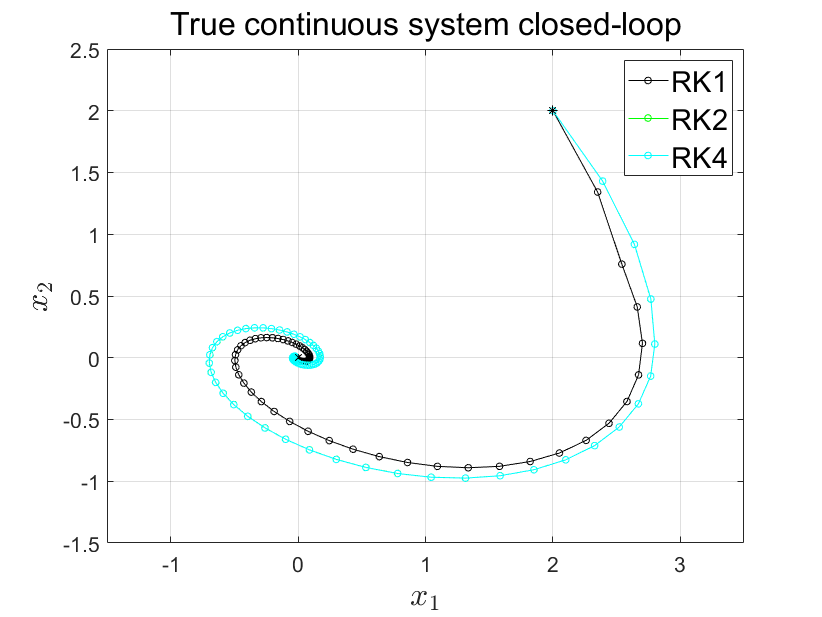
\includegraphics[width=\linewidth]{pics/deltat = 0.04.png}
	\caption{State trajectory of true continuous system}
	\label{fig:statetrajec0.04}
\end{figure}
\newline
In Fig. \ref{fig:statetrajec0.04}, the black line represents the system behavior of RK1 model, while the RK2 has a green line, and it coincides with the cyan line in the plot, which means that the approximation performance between RK2 and RK4 models at a sampling time of $0.04$ seconds is extremely similar.
Now assume that the sampling time $\Delta t = 0.02$ seconds, the corresponding state trajectory of the true system is shown in Fig. \ref{fig:statetrajec0.02}.
\begin{figure}[H]
 	\centering
 	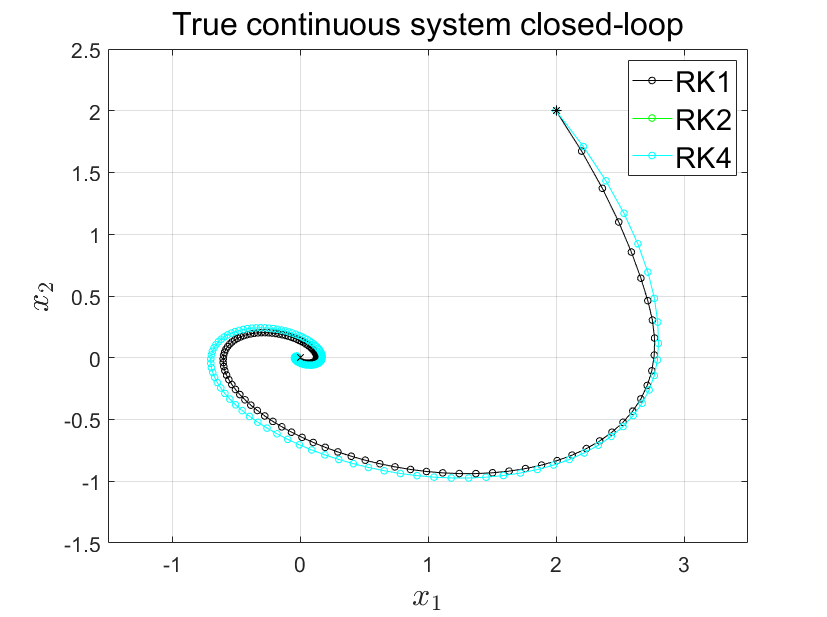
\includegraphics[width=\linewidth]{pics/deltat = 0.02.png}
 	\caption{State trajectory of true continuous system}
 	\label{fig:statetrajec0.02}
\end{figure}

In Fig. \ref{fig:statetrajec0.02}, it can be observed that the black line of RK1 is closer to the green line with a smaller sampling time $\Delta t$, which indicates that the shorter sampling time, the higher the accuracy.
\newline
In Fig. \ref{fig:statetrajec0.020.04}, we apply a smaller sampling time $\Delta t = 0.008$ for RK1 model, while applying a larger sampling time $\Delta t = 0.04$ for RK2 and RK4 models, the state trajectory of three models are extremely similar, which indicates decreasing the sampling time $\Delta t$ of RK1 model so that it has the same accuracy as RK2 and RK4 models with larger sampling time $\Delta t$.
 \begin{figure}[h!]
	\centering
	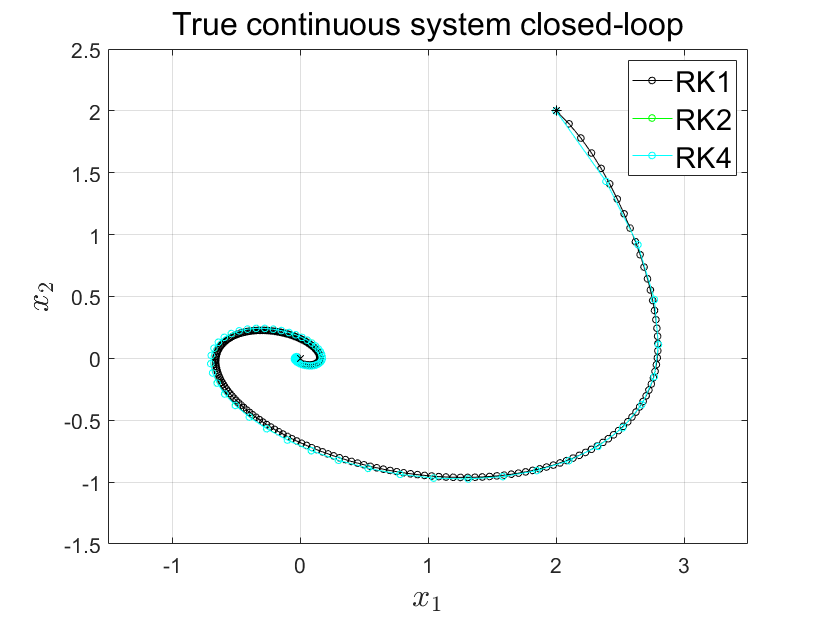
\includegraphics[width=\linewidth]{pics/delta0.04rk10.02rk2rk4.png}
	\caption{State trajectory of true continuous system}
	\label{fig:statetrajec0.020.04}
\end{figure}
\newline
\\
We can achieve similar accuracy between RK1 model with small sampling time and RK4 model with large sampling time, however, this yields increased computational cost due to the increased number of optimization steps. Fig. \ref{fig:timempc} shows the time consumption for RK1 model with sampling time $\Delta t = 0.008$ and RK4 model with sampling time $\Delta t =0.04$ of each MPC iteration.
\begin{figure}[H]
	\centering
	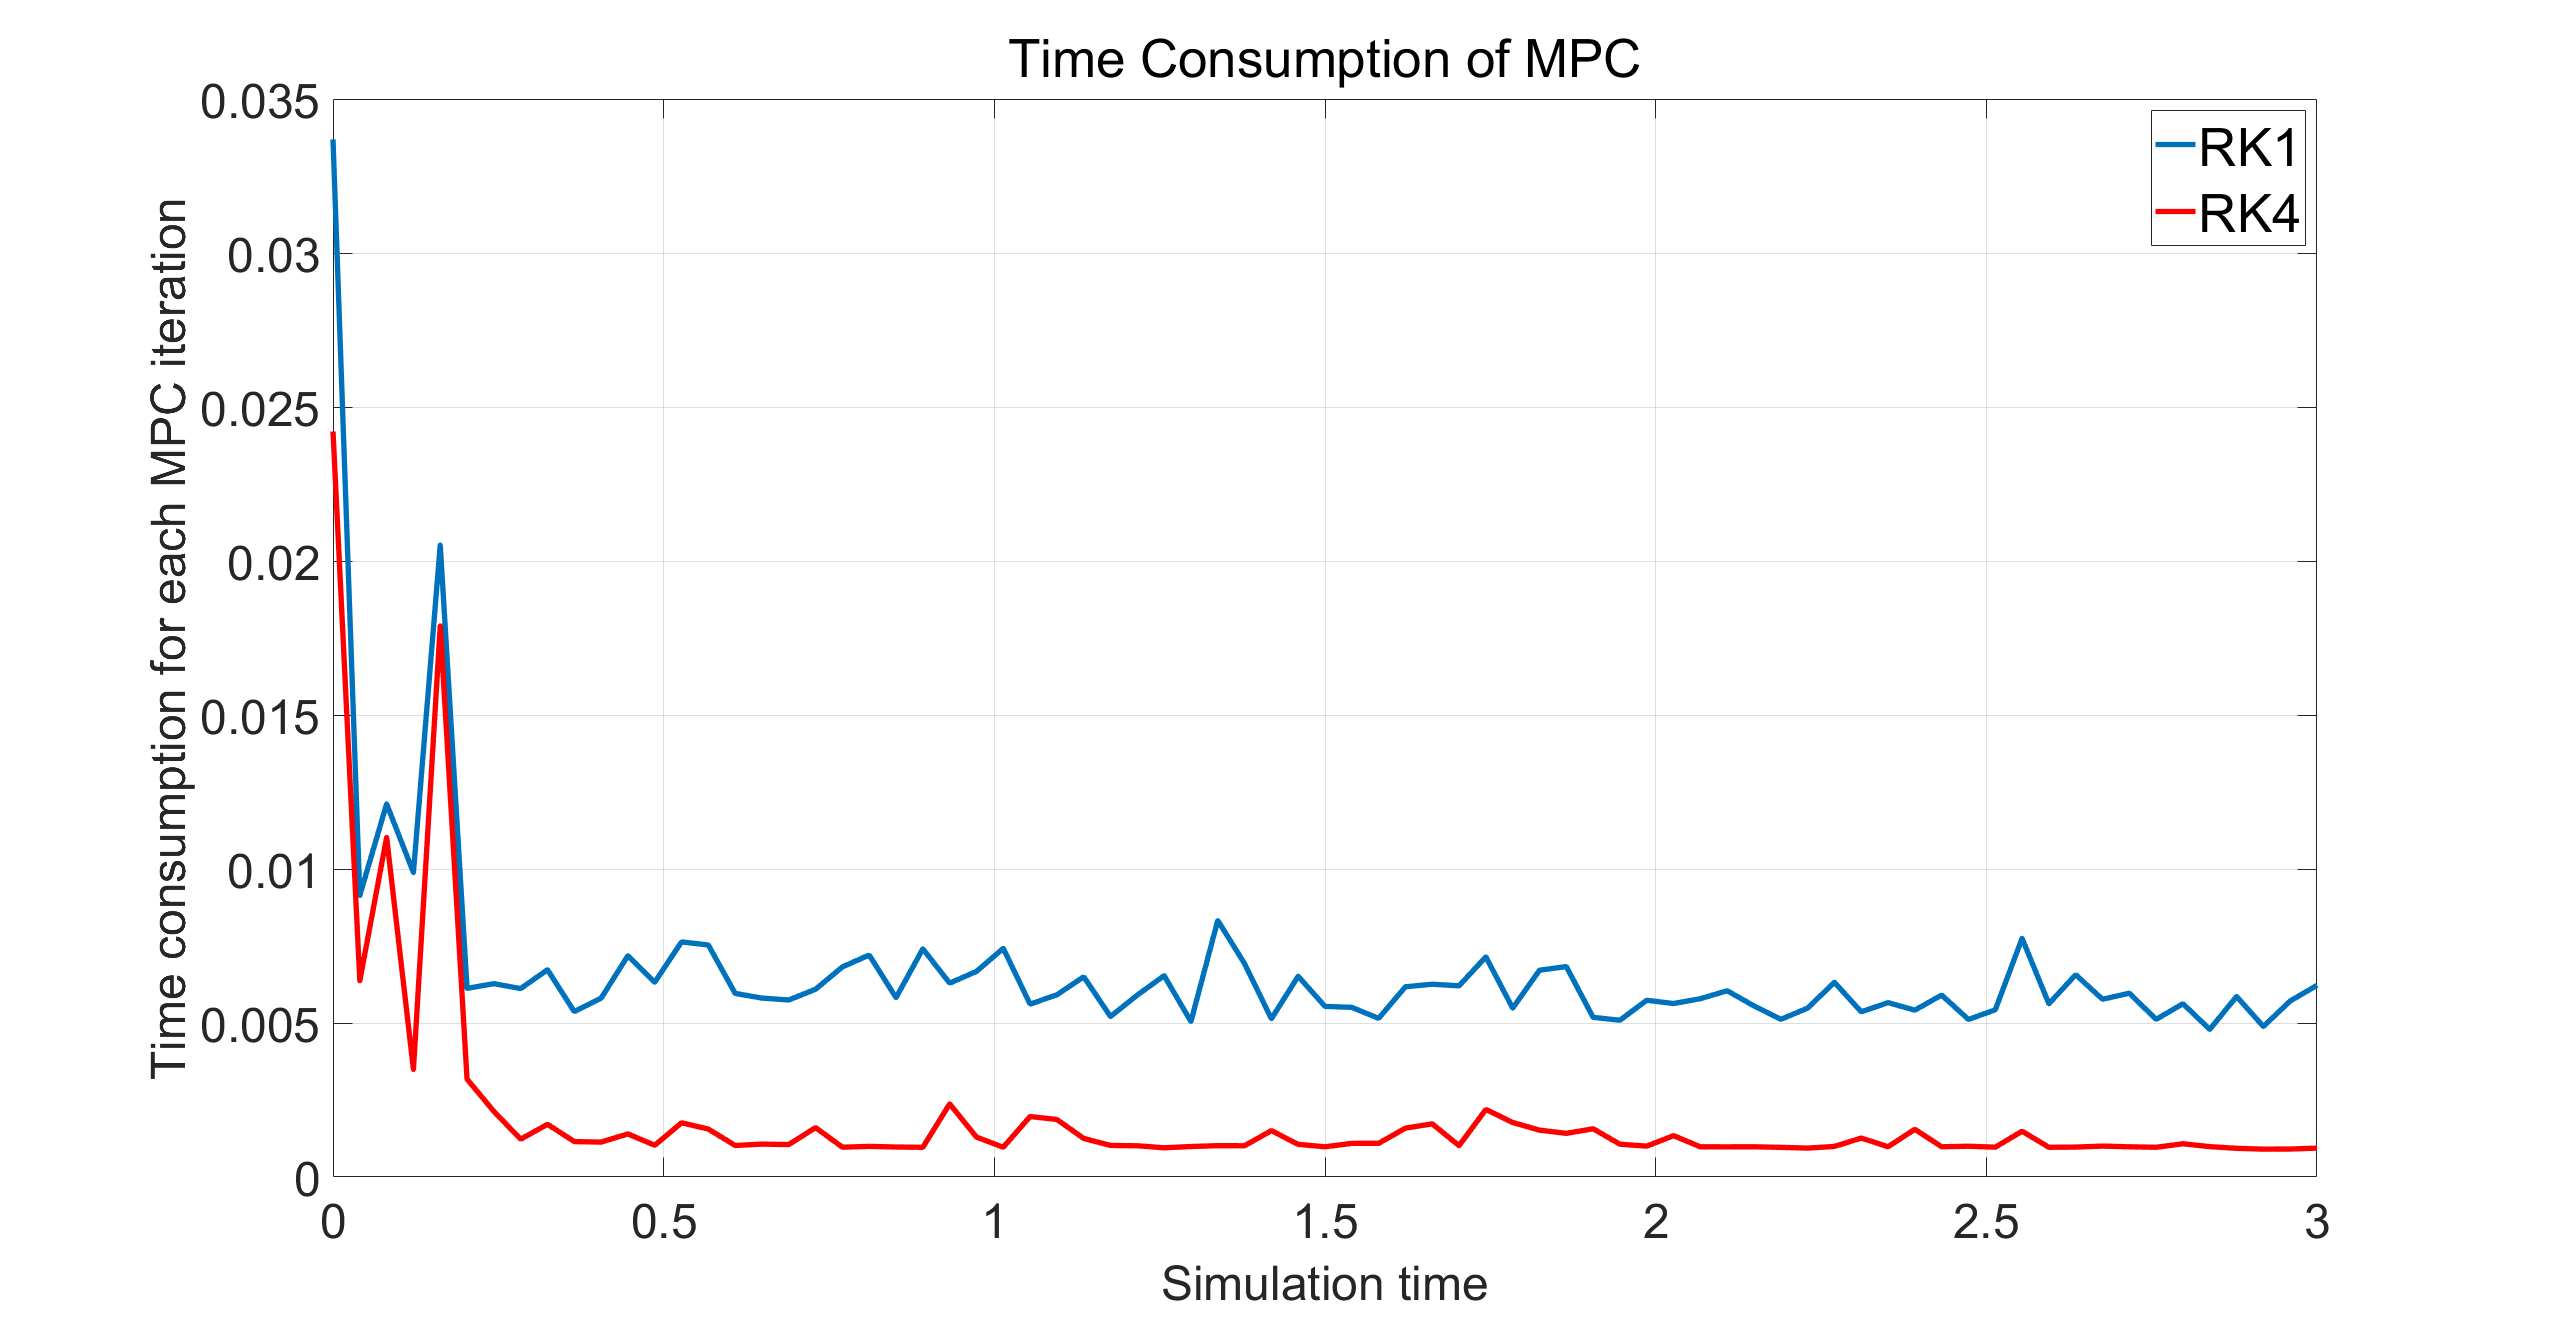
\includegraphics[width=\linewidth]{pics/timempc.png}
	\caption{Time consumption of MPC iteration}
	\label{fig:timempc}
\end{figure}
It is clear that there is a peak in computation time in the first few MPC iterations, which is due to the fact that state $x_1$ here violates the constraint and takes longer to compute the optimal control input $u$.

Next step, we investigates the open-loop performance:
\begin{enumerate}
	\item  Given the continuous time system, apply different discretization methods (RK of different order, and also vary the sampling time/discretization grid) to retrieve different discretized models.
	
	\item Apply an MPC iteration to retrieve an optimal (discrete time) control input sequence.
	
	\item  Apply the control input sequence to the discretized model, and also transform the control input sequence to a continuous time sequence using ZOH and apply it to the true (continuous) system dynamics.
\end{enumerate}
The prediction accuracy of different RK models vary from sampling time, the results shown in Table below
\begin{table}[H]
	\centering
	\begin{tabular}{|c|c|c|c|}
		\hline
		\diagbox{$\Delta$ t}{Error}{RK model}&RK1&RK2&RK4\\ 
		\hline
		0.04&0.323&0.095&0.102\\
		\hline
		0.02&0.081&0.063&0.062\\
		\hline
	\end{tabular}
\end{table}
\begin{equation}
	\epsilon = \frac{\sum_{k=1}^{N} |x_{\rm{con}}(k) - x_{\rm{pre}}(k)|}{N},
\end{equation}
where $N = T/ \Delta t$, $x_{\rm{con}}(k)$ is the true continuous system predicted states at step $k$ and $x_{\rm{pre}}(k)$ is the MPC predicted states at step $k$.

Next, we investigate the control invariant set and the invariant set for the uncontrolled system. Fig. \ref{fig:coninvesetrk1} shows the control invariant set of RK1 and RK4 model with sampling time $\Delta t = 0.06$.
\begin{figure}[H]
	\centering
	\begin{subfigure}[b]{0.37\textwidth}
		\centering
		\includegraphics[width=\linewidth]{pics/coninvset0.06.png}
		\caption{The control invariant set for RK1 model}
		\label{fig:coninvesetrk1}
	\end{subfigure}
	\hfill
	\begin{subfigure}[b]{0.37\textwidth}
		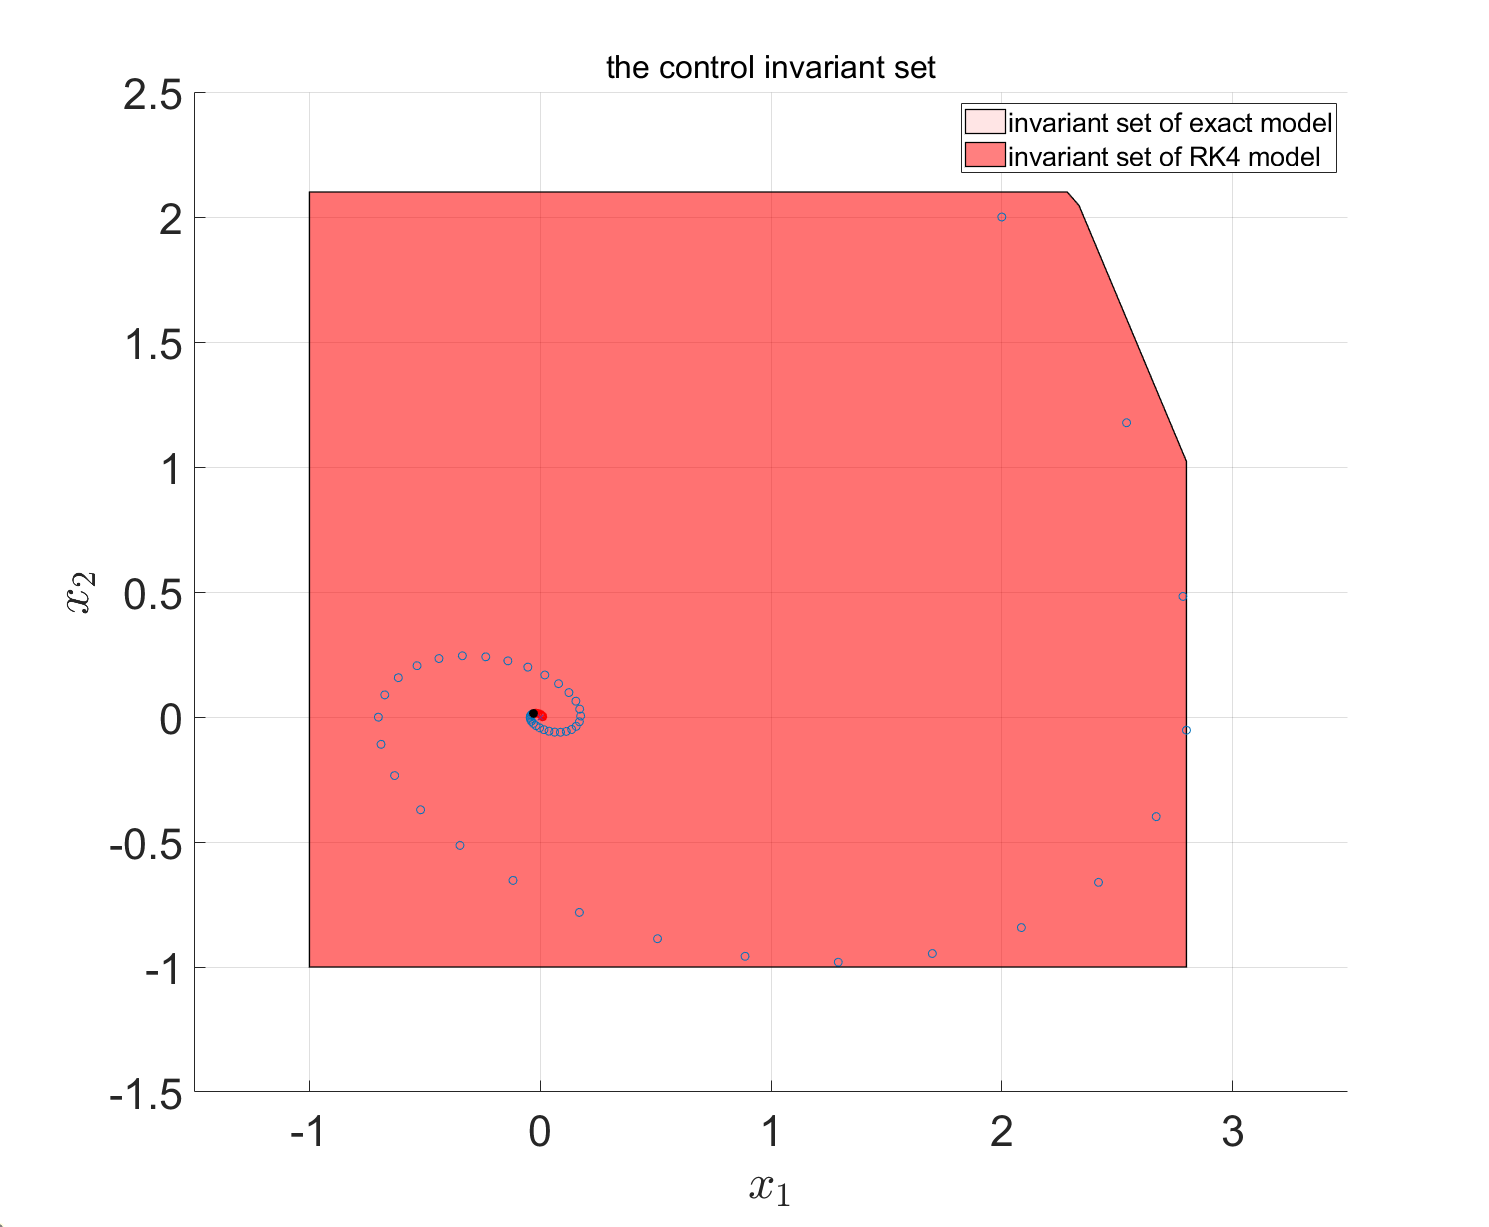
\includegraphics[width=\linewidth]{pics/CONINVSETRK40.06.png}
		\caption{The control invariant set for RK4 model}
		\label{fig:coninvesetrk4}
	\end{subfigure}
    \caption{The control invariant set}
	\label{The control invariant set}
\end{figure}

Compared to the control invariant set of the exact model, the initial state $x_0 = [2,2]^{\top}$ is not in the control invariant set of RK1 model, thus, it is impossible to derive an feasible control input $u$, such that $x_1$ does not violate the state constraint, which indicates the inaccuracy and limitations of the RK1 model.

Fig. \ref{fig:coninvesetrk4} shows the control invariant set of RK4 is the same as the one of exact model, which indicates the higher accuracy compared to RK1 model.

Fig. \ref{fig:invesetrk1} and \ref{fig:invesetrk4} shows the invariant set of RK1 and RK4 model with sampling time $\Delta t = 0.03$.
\begin{figure}[H]
	\centering
	\begin{subfigure}[b]{0.37\textwidth}
		\centering
		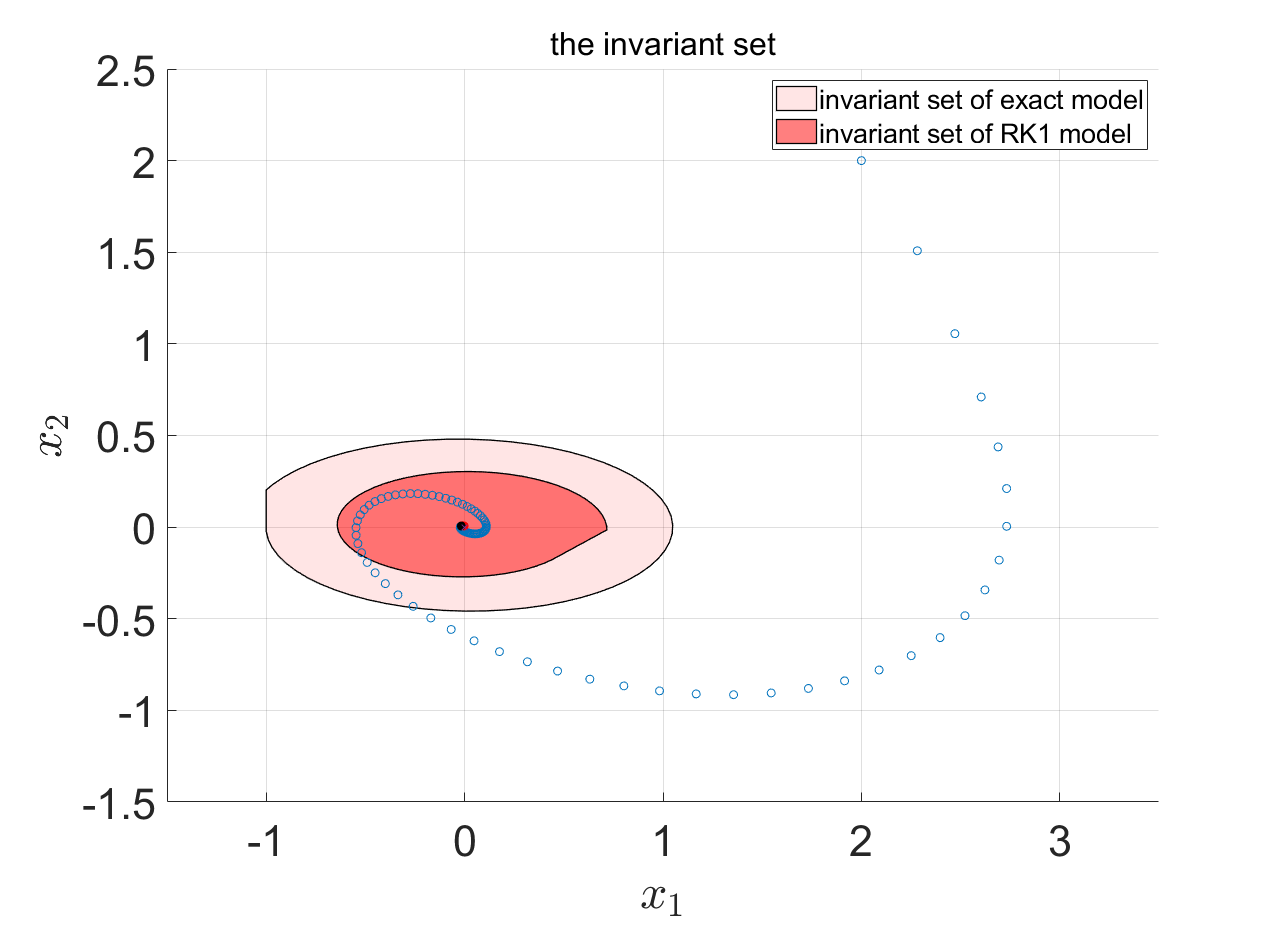
\includegraphics[width=\linewidth]{pics/invsetrk1.png}
		\caption{The invariant set of RK1}
		\label{fig:invesetrk1}
	\end{subfigure}
	\hfill
	\begin{subfigure}[b]{0.37\textwidth}
		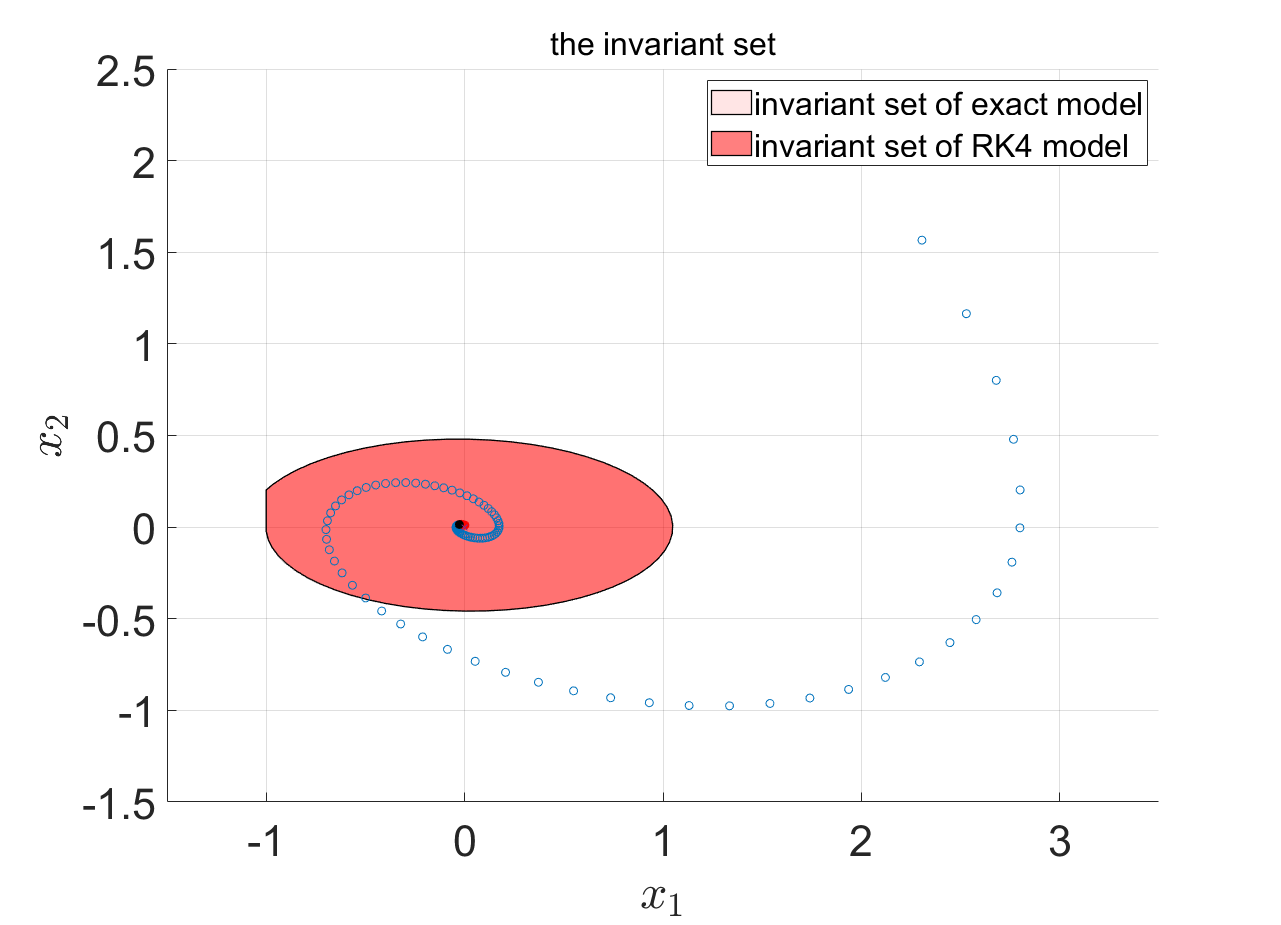
\includegraphics[width=\linewidth]{pics/invsetrk4.png}
		\caption{The invariant set of RK4}
		\label{fig:invesetrk4}
	\end{subfigure}
    \caption{The invariant set}
	\label{fig:The invariant set}
\end{figure}

Similar to the control invariant set, the invariant set for the uncontrolled system of RK1 model is less accurate than the one of RK4 model.
\subsection{Gauss collocation method}
For the Gauss collocation model, the discretized system matrices $A_d$ and $B_d$ are different with different order hold control input $u$. In this example, the ZOH and FOH are implemented. The state trajectory of the Gauss collocation method is compared with the corresponding exact discretized model, whose system matrices are $A_{\rm{ex}}$ and $B_{\rm{ex}}$.

Fig. \ref{fig:gczero.png} shows the state trajectory of exact model and Gauss collocation model with the sampling time $\Delta t = 0.04$ in the case of ZOH. Fig. \ref{fig:ZOHINPUT} shows the corresponding ZOH control input signal.
\begin{figure}[h!]
	\centering
	\begin{subfigure}[b]{0.37\textwidth}
		\centering
		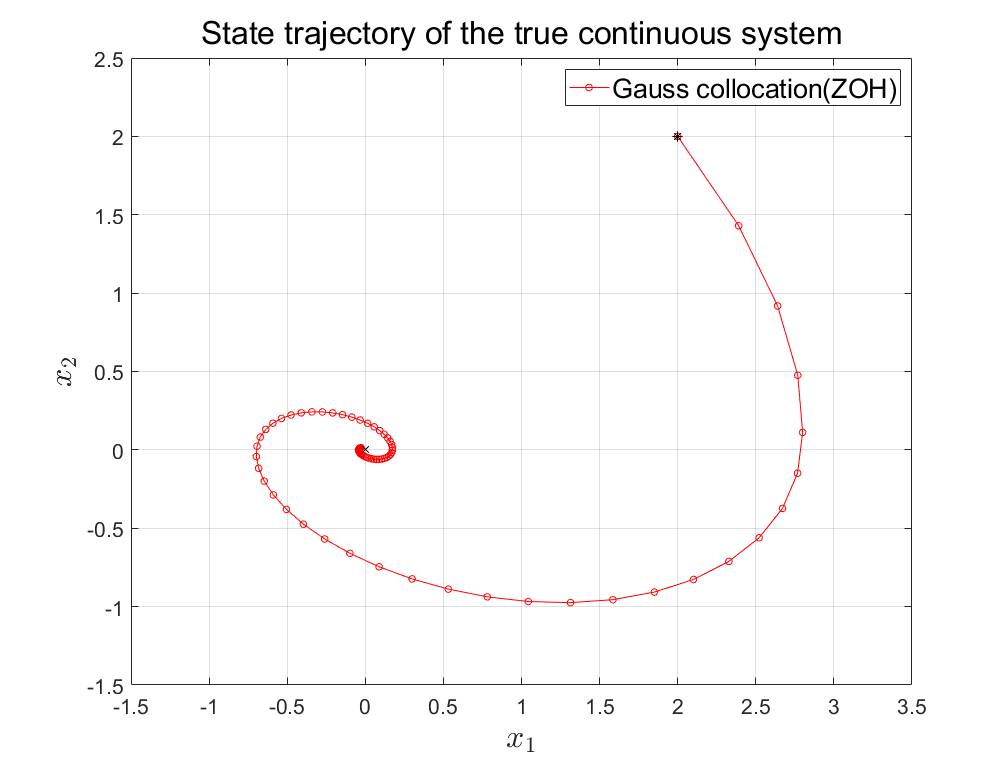
\includegraphics[width=\linewidth]{pics/gczero.png}
		\caption{State trajectory of the true continuous system for ZOH}
		\label{fig:gczero.png}
	\end{subfigure}
	\hfill
	\begin{subfigure}[b]{0.37\textwidth}
		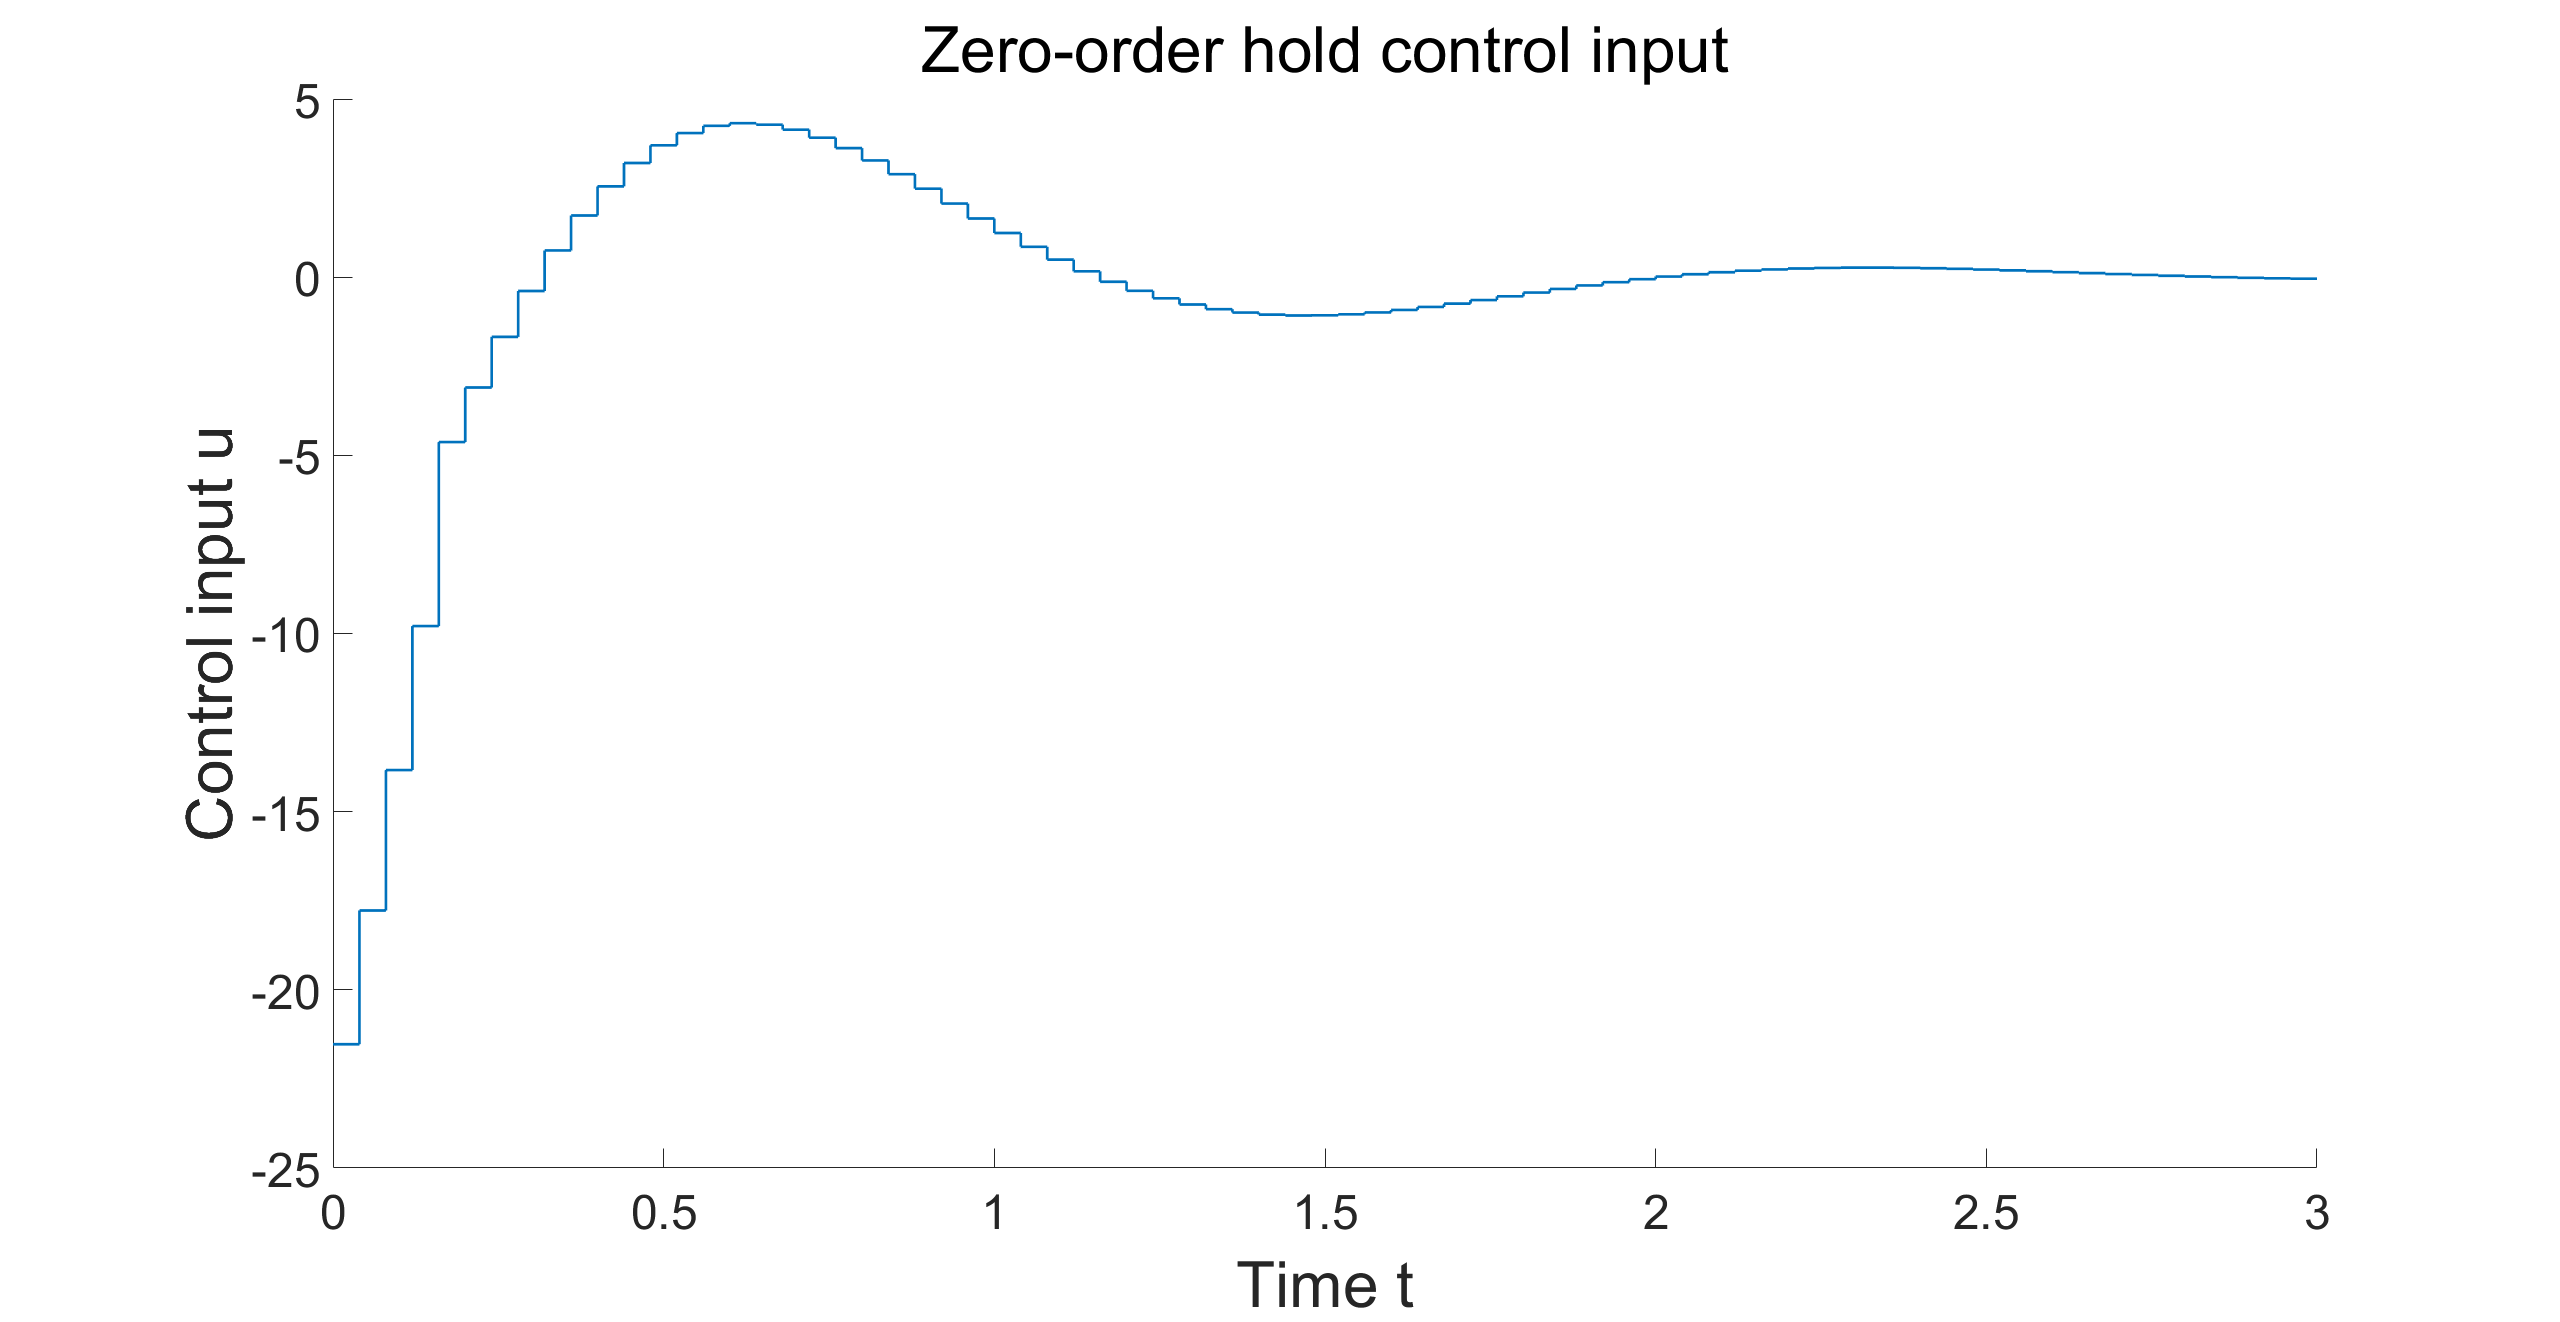
\includegraphics[width=\linewidth]{pics/ZOHINPUT.png}
		\caption{ZOH control input}
		\label{fig:ZOHINPUT}
	\end{subfigure}
	\caption{The state trajectory and ZOH control input}
	\label{fig:The ZOH}
\end{figure}

Fig. \ref{fig:gcfirst.png} shows the state trajectory of exact model and Gauss collocation model with the sampling time $\Delta t = 0.04$ in the case of FOH. Fig. \ref{fig:FOHINPUT} shows the corresponding FOH control input signal.
\begin{figure}[H]
	\centering
	\begin{subfigure}[b]{0.37\textwidth}
		\centering
		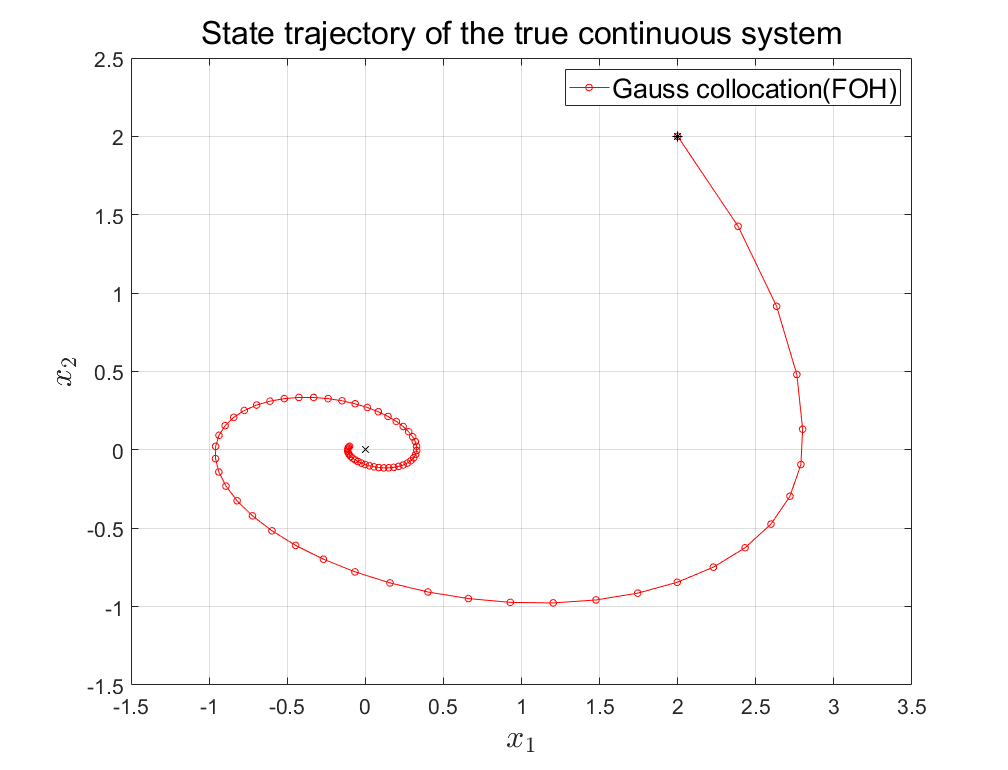
\includegraphics[width=\linewidth]{pics/gcfirst.png}
		\caption{State trajectory of the true continuous system for FOH}
		\label{fig:gcfirst.png}
	\end{subfigure}
	\hfill
	\begin{subfigure}[b]{0.37\textwidth}
		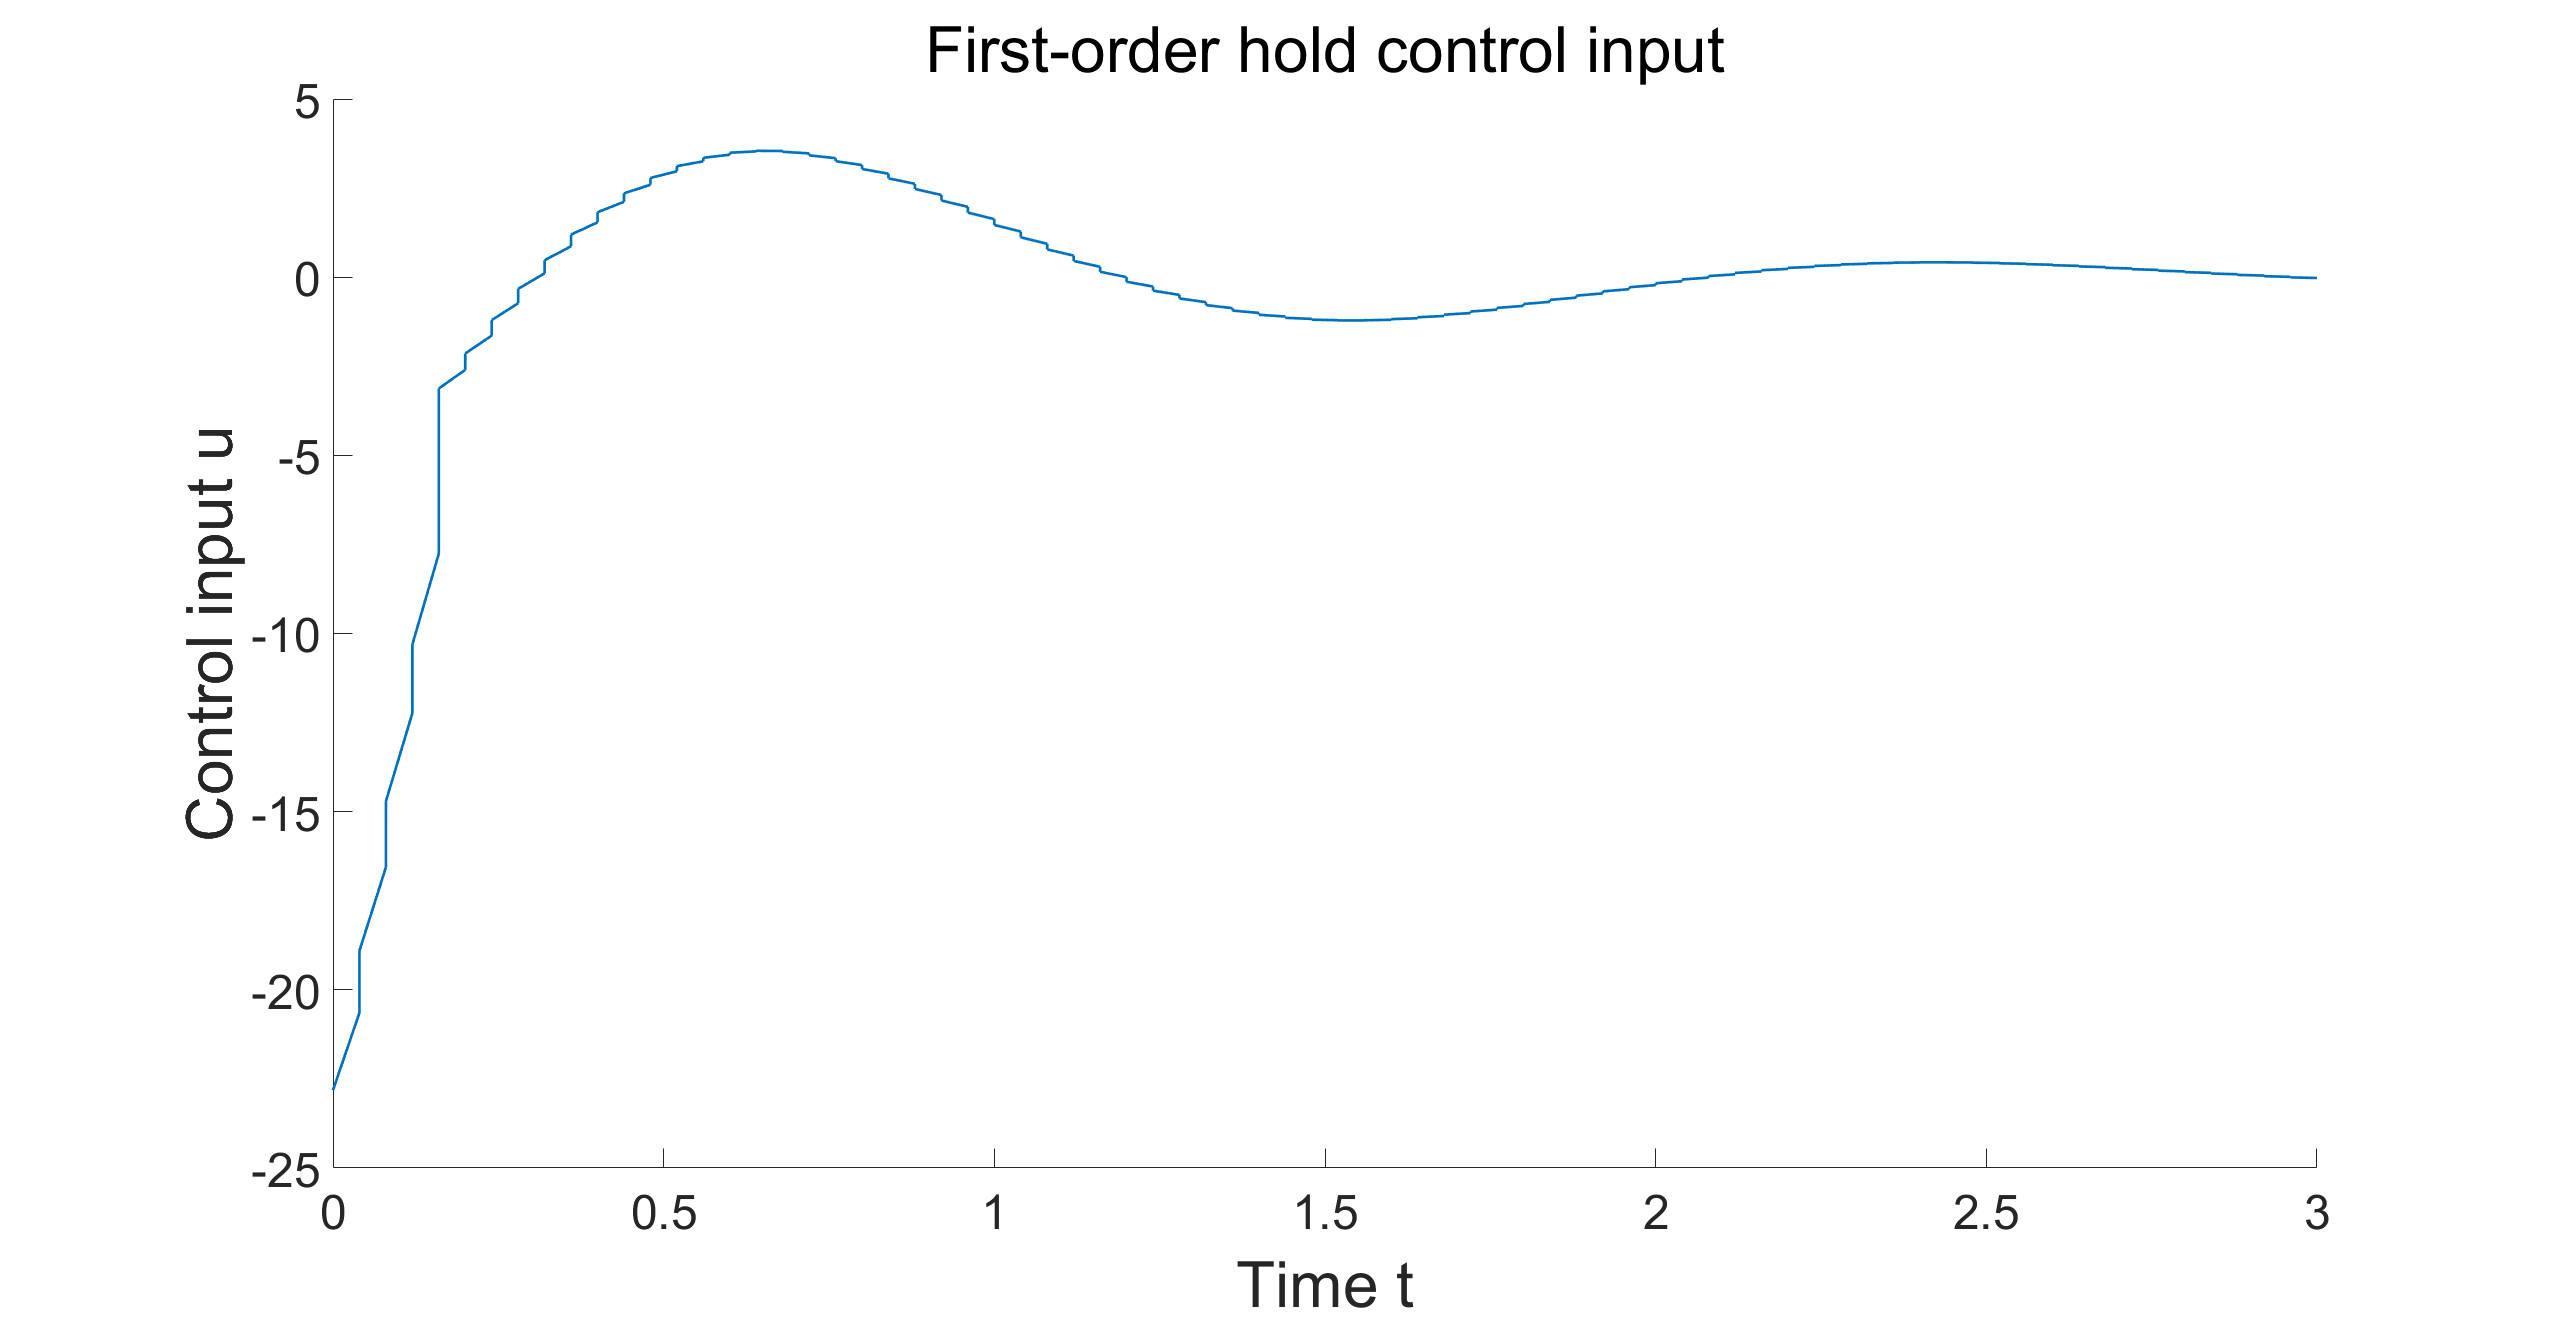
\includegraphics[width=\linewidth]{pics/FOHINPUT.png}
		\caption{FOH control input}
		\label{fig:FOHINPUT}
	\end{subfigure}
	\caption{The state trajectory and ZOH control input}
	\label{fig:The FOH}
\end{figure}
Next, we investigate the control invariant set in case of ZOH and FOH. Fig. \ref{fig:gsconinvset} shows the control invariant set in the case of ZOH control input and FOH control input. It is obvious that the control invariant set of ZOH is a subset of the control invariant set of FOH, which indicates that the MPC solver can find piecewise linear input signals for the whole state set regarding control invariance, while in the case of piecewise constant input signals (ZOH), the control invariant set is decreased.
\begin{figure}[H]
	\centering
	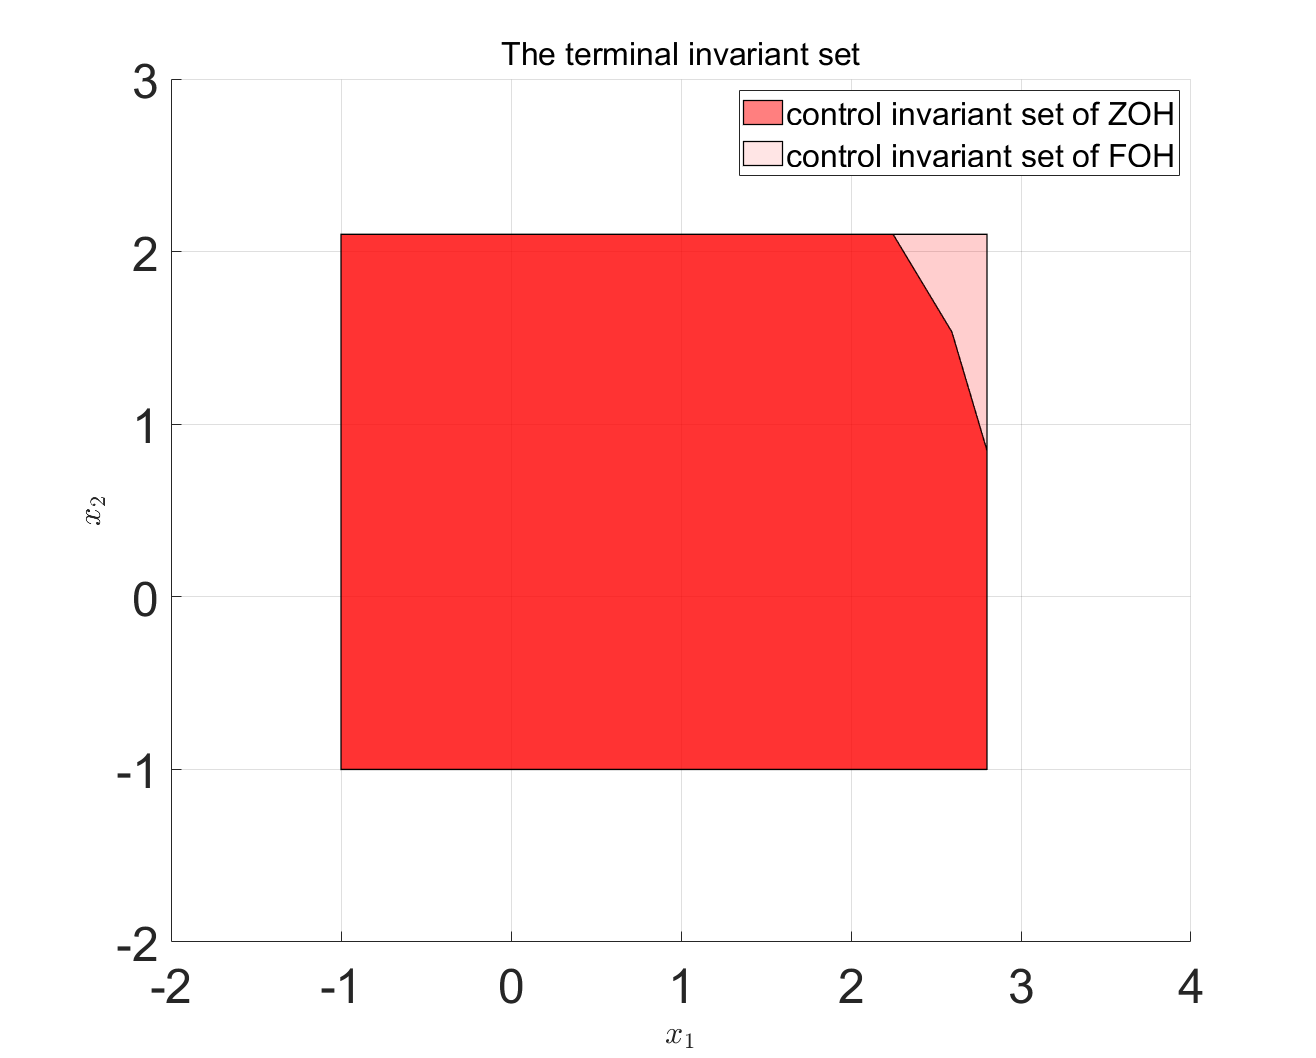
\includegraphics[width=\linewidth]{pics/gcinvariantset.png}
	\caption{The control invariant set}
	\label{fig:gsconinvset}
\end{figure}

 







%_____Zusammenfassung, Ausblick_________________________________
\chapter{Conclusion}
In this work, we compared different discretization methods for a LTI continuous time system. Specifically, we have investigated RK methods of different order and Gauss collocation methods that allow piecewise polynomial input functions within MPC. We have found that the prediction accuracy and closed-loop performance of MPC increased with increasing order of the RK method that is used for discretizing the continuous-time system model. Our simulation example also showed that we can achieve similar accuracy between RK1 with small sampling time and RK4 with large sampling time, however, this yields increased computational cost due to the increased number of optimization variables. For the Gauss collocation method, we investigated the state trajectory for different-order hold control input. It was shown that the control invariant set of FOH control input is larger than ZOH control input, as FOH can consider more input shapes than ZOH.


For future research and further extension, we  can do the same investigation on nonlinear systems, considering even higher-order hold control inputs beyond FOH, e.g., second-order hold. We also found that in Fig. \ref{fig:FOHINPUT} there are big jumps at each sampling instant, it would also be interesting to investigate how to add possible continuity constraint which would be to fix the end point of one interval with the initial point of the following interval. 


%%%%%%%%%%%%%%%%%%%%%%%%%%%%% APPENDIX %%%%%%%%%%%%%%%%%%%%%%%%%%%%%%%%
% APPENDIX
%\appendix
\appendices

%%_________Appendix__________________________________

% final tutorial remarks
\ifLSRITRtutorial
	\chapter{BUSTED! Last chance to actually read the HowTo-Section!}
	
%	Make sure your thesis is well structured, that each major section does what it is supposed to do, and that the whole thing hangs together. The basic structure is often as given in this template (but other structures are possible). In particular, don't think you need to have exactly as many major sections or chapters as the list implies; sometimes it makes sense to merge things, sometimes it makes sense to move things (e.g., the literature review is in many papers deferred until after the results), sometimes it makes sense to split a logical part into several individual sections. Just use some common sense.
%	
%	Hand in your thesis at minimum \textbf{one week} before the deadline for correction. You will receive feedback for the final version and very likely have to do minor or major revisions of your writing. Plan your writing schedule to allow for these adjustments, which can have quite some impact on your grade! 
%	
%	\optional{Please have a look on our \href{https://wiki.lsr.ei.tum.de/thesiswriting_students}{thesis-guidelines} as well before submitting your \emph{final} thesis.}
	
\optional{Do not forget to check our \href{https://wiki.tum.de/display/lsritr/Students}{\underline{thesis-guidelines}} before submitting your \emph{final} thesis.}	
	
%	\section{Style and Expressions}
%	
%	Before handing in your thesis, even for an intermediate review, please perform a spellcheck and correct grammar mistakes. The report is not meant to be a narrative text. Please stick to neutral and technical style and avoid subjective or biased expressions or adjectives/adverbs such as \emph{obviously, always, very, especially well, actually, so-called etc}. Scientific writing is about precision and you should underpin your statements factually, not soften them with unnecessary qualifiers.
%	
%	... Okay enough. But please check chapter \ref{sec:Tutorial} before starting with your report. 

\section{Spellcheck reminder}
Before handing in your thesis, even for an intermediate review, please perform a proper spellcheck and correct grammar mistakes. Otherwise, there is a high likelihood that your supervisor will return your report immediately without making any comments.
\fi

%%%%%%%%%%%%%%%%%%%%%%%%% References %%%%%%%%%%%%%%%%%%%%%%%%%%%%%%%%%
\bibliography{refs/mybib}
\bibliographystyle{ieeetr}


%%%%%%%%%%%%%%%%%%%%%%%%% List of Abrevations %%%%%%%%%%%%%%%%%%%%%%%%%%%%%%%%%

\end{document}
